\documentclass[conference]{IEEEtran}
\IEEEoverridecommandlockouts

\usepackage{cite}
\usepackage{amsmath,amssymb,amsfonts}
\usepackage{algorithmic}
\usepackage{graphicx}
\usepackage{textcomp}
\usepackage{booktabs}
\usepackage{multirow}
\usepackage{url}

\usepackage[table]{xcolor}
\usepackage{makecell}
\usepackage{algorithm}
\usepackage{algorithmic}
\newcommand{\bench}{EviStateBench}
\newcommand{\engine}{EviStateDB}
\newcommand{\tsv}{TemporalStateView}

\usepackage{xspace}
\newcommand{\parab}[1]{\vspace{0.01in}\noindent{\bf #1} }
\newcommand{\first}{\textsf{(i)}\xspace}
\newcommand{\second}{\textsf{(ii)}\xspace}
\newcommand{\third}{\textsf{(iii)}\xspace}
\newcommand{\fourth}{\textsf{(iv)}\xspace}
\newcommand{\fifth}{\textsf{(v)}\xspace}
\newcommand{\sixth}{\textsf{(vi)}\xspace}
\newcommand{\seventh}{\textsf{(vii)}\xspace}
\newcommand{\zzm}[1]{\textcolor{magenta}{\textbf{zzm:} #1}}
\newcommand{\sys}{\textsf{Trident}\xspace}
\newcommand{\detect}{\textsf{tSieve}\xspace}
\newcommand{\outlier}{\textsf{tScissors}\xspace}
\newcommand{\cluster}{\textsf{tMagnifier}\xspace}
\newcommand{\etc}{\emph{etc.}\xspace}
\newcommand{\ie}{\emph{i.e.,}\xspace}
\newcommand{\eg}{\emph{e.g.,}\xspace}
\newcommand{\cf}{\emph{c.f.,}\xspace}
\newcommand{\etal}{\emph{et al.}\xspace}


\begin{document}

\title{[Experiment, Analysis, and Benchmark] EviStateBench: A Benchmark for Temporal Task-State View Maintenance over Embodied Observation Streams}

\iffalse
\author{\IEEEauthorblockN{ and }
\IEEEauthorblockA{Zhejiang University, China\\
\{22421190,22421168\}@zju.edu.cn}}
\fi

\author{Jiaxiang Zhou\textsuperscript{1},
Yizheng Huang\textsuperscript{1},
Yiqun Zhou\textsuperscript{1},
Ziming~Zhao\textsuperscript{1}\\
\textsuperscript{1}Zhejiang University, Hangzhou, China\\
\{jiaxiang, Yizhengz, yiqunz, zhaoziming\}@zju.edu.cn
}



\maketitle

\begin{abstract}
Embodied agents produce observation streams from perception modules, action logs, trackers, task monitors, and simulators. These streams are often noisy, delayed, out of order, incomplete, and contradictory. Downstream task execution, however, needs queryable task-state views with temporal validity, information-availability semantics, uncertainty, and provenance: whether an object was inside a container at a valid time, whether that fact was known before late evidence arrived, which observations support or contradict it, and whether task goals currently hold. Existing embodied benchmarks mainly evaluate task completion, navigation, question answering, or memory recall; they do not isolate this data-management workload. We present \bench, an Experiment, Analysis, and Benchmark contribution for temporal task-state view maintenance over embodied observation streams. \bench\ constructs hidden state timelines from simulator truth and task specifications, releases sanitized StateObservation streams as public input, and evaluates standardized QueryAnswer predictions against hidden answer sets. Its workload covers bitemporal state, provenance, change sets, uncertainty sets, preconditions, failure localization, and goal-state queries. The reported artifact contains 570 simulator-grounded episodes from 36 activities, 5,848 hard queries, 2.86M clean observations, and 2.80M hard mixed observations; public-artifact, query-semantics, and answer-schema validation all pass. We also provide \engine, a reference baseline that materializes bitemporal task-state views with support and contradict evidence. Experiments with recall-memory, temporal-log, and \engine\ baselines show that \bench\ separates retrieval, log-based lookup, and materialized temporal-state maintenance: exact accuracy ranges from 25.2\% to 75.6\%. The remaining errors concentrate in structured, set-valued, and task-derived queries, identifying open stress points for data systems over embodied evidence streams.
\end{abstract}

\begin{IEEEkeywords}
Benchmarking, Temporal Data Management, Bitemporal Data, Stream Processing, Incremental View Maintenance, Embodied AI
\end{IEEEkeywords}


\section{Introduction}

Embodied agents increasingly observe the world through streams rather than through clean symbolic states. A robot may receive a detector output that a cabinet is open, a relation estimate that a cup is inside the cabinet, an action log that a place operation succeeded, and a later visual observation that contradicts the earlier relation. These records may come from different sources, arrive at different times, and have different reliability. Some describe the current world state, while others arrive late and refer to an earlier event. Some evidence is missing because an object was occluded; some evidence is wrong because perception failed. A task executor nevertheless needs database-like answers: does the goal hold now, what would the system have known at a previous transaction time, which states changed during the episode, and which observations support or contradict an answer?

This is a data-management problem that is not isolated by current embodied benchmarks. BEHAVIOR introduced household activities with predicate-logic initial and goal conditions~\cite{srivastava2022behavior}, while BEHAVIOR-1K scales this setting to long-horizon mobile manipulation in a richer simulation environment~\cite{li2024behavior1k}. Habitat and Habitat 2.0 support embodied navigation and rearrangement evaluation~\cite{savva2019habitat,szot2021habitat}. AI2-THOR provides an interactive 3D environment for visual AI~\cite{kolve2017ai2thor}, and VirtualHome represents household activities as executable programs~\cite{puig2018virtualhome}. TEACh studies embodied agents that interact through dialogue~\cite{padmakumar2022teach}. OpenEQA evaluates open-vocabulary embodied question answering over episodic memory and active exploration~\cite{majumdar2024openeqa}, and ALFRED evaluates grounded instruction following for everyday tasks~\cite{shridhar2020alfred}. These benchmarks expose important task, language, perception, navigation, and interaction challenges. Their primary scoring target, however, is not whether a data system can maintain a temporal task-state view from imperfect public observation streams with valid-time semantics, transaction-time availability, uncertainty, provenance, and structured query workloads.

The distinction matters for database systems. In a task such as placing a cup into a cabinet and closing the door, the relevant maintained states may include \texttt{inside(cup,cabinet)}, \texttt{open(cabinet)}, and \texttt{grasped(robot,cup)}. The query \emph{was the cup inside the cabinet after the place action?} is not simply a nearest-frame retrieval query; it is a temporal state query over evidence. The query \emph{what changed between the beginning and end of the episode?} is not a single symbolic-state lookup; it is a change-set query over a maintained view. The query \emph{would the system have known this before the delayed observation arrived?} requires event time and arrival time to be separated, a distinction central to temporal data management~\cite{snodgrass1999developing,jensen1999temporal}. Since observations arrive continuously and may be processed out of order, the workload also inherits concerns from stream processing~\cite{babcock2002models}. Because task-state views must be updated after new evidence, corrections, and late arrivals, it is naturally related to incremental view maintenance~\cite{gupta1995maintenance,zhuge1995view}. Finally, because evidence can be incomplete, noisy, or contradictory, the benchmark connects to uncertain data and provenance-aware data management~\cite{aggarwal2009uncertain,green2007provenance,cheney2009provenance}.

We introduce \bench, a data-management benchmark for temporal task-state view maintenance over embodied observation streams. A \bench\ task instance provides public task specifications, StateObservation streams, queries, and metadata. It withholds hidden state timelines and hidden answer sets used by the evaluator. Systems under test may use any internal representation, including retrieval memory, temporal logs, SQL scans, rules, materialized views, learned memory, or hybrids. They are compared only through standardized QueryAnswer predictions under a shared evaluator. This public/hidden split is central to the benchmark: the oracle is derived from simulator truth and task specifications, not from any submitted system or reference implementation.

The reported \bench\ artifact contains 570 simulator-grounded episodes over 36 activities, 5,848 hard queries, 2.86M clean observations, and 2.80M hard mixed observations. The workload covers bitemporal state, provenance, change sets, uncertainty sets, preconditions, failure localization, and task-goal queries. Public-artifact validation, query-semantics audit, and answer-schema validation pass without errors. Experiments with recall-memory, temporal-log, and materialized temporal-state baselines show that the benchmark separates retrieval-style memory, log-based temporal lookup, and explicit temporal view maintenance: exact accuracy ranges from 25.2\% to 75.6\%, while structured, set-valued, and task-derived queries remain difficult.

We also provide \engine, a reference baseline engine for \bench. \engine\ maintains a \tsv\ with valid-time intervals, transaction-time revisions, support and contradict evidence, confidence, and task-derived views. It is useful for diagnosing what an explicit temporal view-maintenance engine can do under the benchmark, but it is not the benchmark oracle. This separation lets \bench\ evaluate \engine\ alongside simpler or future systems under the same public inputs, hidden answers, and scoring protocol.

This paper makes four contributions.
\begin{itemize}
    \item We formulate temporal task-state view maintenance over embodied observation streams as a data-management benchmark problem, separating it from perception, control, task completion, and memory-recall evaluation.
    \item We define the \bench\ artifact boundary, StateObservation schema, query workloads, perturbation regimes, QueryAnswer schema, and evaluator semantics for public-input/hidden-oracle evaluation.
    \item We describe a simulator-grounded generation pipeline that produces hidden state timelines, clean and perturbed public observation streams, query sets, hidden answer sets, validation reports, and reproducible benchmark manifests.
    \item We provide \engine\ as a reference baseline engine and an experimental protocol for comparing retrieval, log-based, and materialized temporal-state maintenance strategies under shared public inputs and hidden oracle answers.
\end{itemize}

The intended EAB contribution is therefore not a new perception model, planner, or robotics controller. It is the benchmark object: a standardized artifact, a diagnostic query workload, a public/hidden evaluation boundary, an evaluator, and an analysis protocol for systems that maintain temporal task-state views. This follows the tradition of database benchmark papers such as LDBC for graph workloads~\cite{erling2015ldbc,iosup2016ldbc}, TSM-Bench for time-series systems~\cite{khelifati2023tsmbench}, and FinBench for financial graph transaction workloads~\cite{qi2025finbench}. It also aligns with recent EAB work that contributes evaluation frameworks and diagnostic analyses, including SQLMorph~\cite{malekpour2026sqlmorph}, BEACON~\cite{najafi2025beacon}, and plan-based AQP analysis~\cite{mu2025aqp}.



\begin{table*}[!t]
\caption{Benchmark positioning. Existing embodied benchmarks evaluate task execution, simulation, instruction following, question answering, or memory recall. \bench\ isolates temporal task-state view maintenance from imperfect observation streams.}
\label{tab:related-benchmarks}
\centering
\scriptsize
\newcommand{\yes}{\checkmark}
\newcommand{\no}{--}
\newcommand{\partly}{Partial}
\setlength{\tabcolsep}{2.4pt}
\renewcommand{\arraystretch}{1.15}
\begin{tabular}{ccc c c c c}
\toprule
\textbf{Benchmark family} & \textbf{Primary target} & \makecell{\textbf{Temporal}\\\textbf{state queries}} & \makecell{\textbf{Event/}\\\textbf{arrival time}} & \makecell{\textbf{Perturbed}\\\textbf{observations}} & \makecell{\textbf{Task-derived}\\\textbf{views}} & \makecell{\textbf{Hidden}\\\textbf{oracle}} \\
\midrule
BEHAVIOR / BEHAVIOR-1K & Household task execution and simulation & \partly & \no & \no & \partly & Simulator truth \\
ALFRED & Instruction following & \no & \no & \no & Task success & Demo labels \\
OpenEQA & Embodied question answering & Episodic context & \no & \no & NL answers & Human/LLM scoring \\
Retrieval memory evals & Recall from stored observations & Limited & \no & Usually no & \no & Dataset labels \\
\rowcolor{gray!10}
\bench & Temporal task-state view maintenance & \yes & \yes & \yes & \yes & Simulator truth + specs \\
\bottomrule
\end{tabular}
\vspace{0.3em}
\begin{flushleft}
\scriptsize
\textit{Note:} \checkmark\ indicates that the property is explicitly evaluated as a first-class scoring target; ``Partial'' indicates that the property may appear in task definitions or simulator state but is not the primary evaluation target.
\end{flushleft}
\end{table*}


\section{Motivation and Benchmark Scope}
\label{sec:motivation}

\subsection{A Running Task-State Example}

Consider a household task in which an agent must put a cup into a cabinet and then close the cabinet. The task can be described by predicates over objects and time: the cup should become \texttt{inside(cup,cabinet)}, the cabinet should eventually be not \texttt{open(cabinet)}, and the robot should no longer be \texttt{grasped(robot,cup)}. A simulator or action script can provide the underlying state changes, but a deployed system observes only a stream of partial evidence. A relation detector may report \texttt{inside(cup,cabinet)} with moderate confidence after the place action. A visual detector may miss the cup once it becomes occluded. An action log may assert that the place operation succeeded. A later observation may arrive after the close action and revise an earlier belief.
This example separates three objects that are often conflated. The \emph{world state} is what actually holds at a valid time. The \emph{observation evidence} is what a source claims, possibly late, incomplete, or incorrect. The \emph{maintained task-state view} is what a system can answer after ingesting the public stream. \bench\ evaluates the third object against hidden answers derived from the first object, while exposing only the second object as public input.

\subsection{What the Benchmark Evaluates}

\bench\ evaluates systems that maintain queryable temporal views of task state. A benchmark instance provides a task specification, an observation stream, and a query set. A system outputs predicted answers, and the evaluator scores them against hidden answer sets. The system is not required to expose its internal state representation. It may use a log scan, a materialized view, relational tables, a retrieval index, rules, a learned memory module, or a hybrid architecture. The only required output is the standardized predicted QueryAnswer.
The workload targets eight query families. \texttt{CHECK\_STATE} and \texttt{CHECK\_GOAL} are compact point probes over task predicates and goal conditions. \texttt{AS\_OF\_STATE} asks what would be known for a valid time at a specified transaction time, thereby testing information-availability semantics under late evidence. \texttt{WHY\_STATE} asks for supporting or contradicting evidence. \texttt{STATE\_DIFF} asks which states changed between two valid-time points or intervals. \texttt{FIND\_UNCERTAIN\_STATES}, \texttt{CHECK\_PRECONDITION}, and \texttt{FAILURE\_LOCALIZATION} expose set-valued uncertainty, task-precondition reasoning, and failure-analysis views.

\subsection{What the Benchmark Deliberately Excludes}

\bench\ is not a robot-control benchmark. It does not score low-level manipulation success, exploration policy, path planning, visual perception quality, or language-grounded action execution as primary outcomes. These components are important, but including them in the main score would make failures difficult to attribute. An accuracy difference could reflect a detector, controller, simulator rollout, or planner rather than the temporal state-maintenance method being evaluated.
The main artifact therefore uses simulator-grounded hidden timelines and controlled public observation streams. This choice is a scope restriction, not a claim that perception and control are unimportant. It makes the stream, queries, hidden answers, and evaluation semantics stable enough to evaluate temporal view maintenance reproducibly. Action-source and perception-source gaps are reported as limitations; the main correctness claim is over the controlled data-management workload.

\subsection{Benchmark Requirements}

The running example yields five benchmark requirements.
\first \emph{R1: Temporal semantics.} The benchmark must ask about current and historical task states, not only final task success.
\second \emph{R2: Information availability.} It must separate valid time from arrival time, so that late evidence can repair a previous state without giving systems credit for knowing it before it arrived.
\third \emph{R3: Evidence sensitivity.} It must represent support and contradict observations, because task states can be uncertain or conflicting under imperfect evidence.
\fourth \emph{R4: Task-derived views.} It must evaluate predicates in the context of task goals, preconditions, changes, and failure explanations, not only isolated object attributes.
\fifth \emph{R5: Reproducibility.} It must provide public inputs, hidden answers, validation reports, and a shared evaluator so that systems are compared under the same workload and scoring semantics.
Table~\ref{tab:related-benchmarks} positions these requirements against related benchmark families. The point is not that prior benchmarks are deficient for their own goals. Rather, they target different layers of the embodied stack. \bench\ fills the data-management layer between observation-producing embodied systems and task executors that need queryable, auditable state.


\section{Problem Definition}
\label{sec:problem}

\subsection{Episodes and Hidden State Timelines}

An episode $e$ is an execution instance of a task specification. A task specification defines the relevant objects, task-state predicates, initial conditions, goal conditions, and task-level metadata. Let $\mathcal{P}$ be the set of task-state predicates, such as \texttt{open}, \texttt{inside}, \texttt{toggled\_on}, \texttt{covered}, \texttt{cooked}, \texttt{temperature}, \texttt{frozen}, and \texttt{attached}. A state atom has the form $p(\mathbf{a})=v$, where $p\in\mathcal{P}$, $\mathbf{a}$ is a tuple of object identifiers or values, and $v$ is a Boolean, categorical, or numeric value.
For each episode, the generator constructs a hidden state timeline
\begin{equation}
    H_e = \langle h_1,\ldots,h_m\rangle ,
\end{equation}
where each event $h_i$ records a state atom, its value, and either a valid-time interval or a transition time derived from simulator truth and the task specification. Hidden timelines are not part of the public input. They are used only to derive hidden answer sets for evaluation.

\begin{table}[!t]
\caption{Query workloads in \bench.}
\label{tab:query-workloads}
\centering
\scriptsize
\setlength{\tabcolsep}{2.4pt}
\renewcommand{\arraystretch}{1.13}
\begingroup
\rowcolors{2}{gray!4}{white}
\begin{tabular}{@{}p{0.31\linewidth}p{0.28\linewidth}p{0.33\linewidth}@{}}
\toprule
\rowcolor{gray!15}
\textbf{Query family} & \textbf{Main input} & \textbf{Evaluated capability} \\
\midrule
\texttt{CHECK\_STATE} & Predicate, arguments, valid time & Point state lookup over task predicates \\
\texttt{AS\_OF\_STATE} & Predicate, valid time, transaction time & Bitemporal availability and repair \\
\texttt{WHY\_STATE} & Predicate, time, evidence scope & Provenance and evidence support \\
\texttt{STATE\_DIFF} & Scope, start time, end time & Change-set maintenance over an episode \\
\texttt{CHECK\_GOAL} & Goal spec, valid time & Task-derived goal view correctness \\
\texttt{FIND\_UNCERTAIN\_STATES} & Episode and state scope & Set-valued uncertainty tracking \\
\texttt{CHECK\_PRECONDITION} & Task state and precondition scope & Task-derived precondition reasoning \\
\texttt{FAILURE\_LOCALIZATION} & Goal subset and state scope & Failed-goal state localization \\
\bottomrule
\end{tabular}
\endgroup
\end{table}

\subsection{Public Evidence Streams and Logical Views}

The public input is a sequence of StateObservations. Each observation is an evidence record
\begin{equation}
\begin{aligned}
o = (&obs\_id, episode\_id, event\_time, arrival\_time, source,\\
     &kind, predicate, arguments, value, confidence,\\
     &polarity, evidence\_ref, metadata).
\end{aligned}
\end{equation}
The \emph{event time} is the time in the episode to which the observation refers. The \emph{arrival time} is the time at which the system receives the observation. The two may differ, which creates the need for transaction-time semantics. The \emph{polarity} indicates whether the observation supports, contradicts, or corrects a state claim. The \emph{evidence reference} links the observation to an artifact item, such as a frame identifier, trajectory identifier, source record, or simulator-derived annotation.
Observation streams can be clean or perturbed. Clean streams contain simulator-derived evidence with minimal injected noise. Perturbed streams introduce missing observations, temporal disorder, low-confidence evidence, and contradictions. The reported release includes a target-aware hard mixed stream that combines these issues and serves as the primary stress condition.

The event-time/arrival-time distinction is central. If an observation with $event\_time=10$ arrives at $arrival\_time=40$, then a system answering at transaction time 20 should not be credited for using it. The same system answering at transaction time 50 may use that observation to repair the maintained view. Thus, valid time describes the modeled world, while transaction time describes information availability. In embodied streams, this mismatch arises naturally from delayed model inference, batch perception, communication delays, and post-hoc task-monitor updates.
A \tsv\ is the logical object being evaluated. For an episode, it can be viewed as a maintained relation
\begin{equation}
\begin{aligned}
V = (&state\_id, episode\_id, predicate, arguments, value,\\
     &valid\_start, valid\_end, transaction\_start,\\
     &transaction\_end, confidence, support, contradict,\\
     &status, revision\_history).
\end{aligned}
\end{equation}
Valid-time fields record when a state is believed to hold in the world. Transaction-time fields record when the system knew or stored that belief. The support and contradict sets record evidence used in the maintained answer. A system under test is not required to materialize $V$ or expose it. The relation defines the benchmark semantics, not an implementation requirement.

\subsection{Queries and Answer Schema}

A query $q$ is a public request over an episode, a predicate or task-goal specification, and one or more time parameters. The main query families are shown in Table~\ref{tab:query-workloads}. Hidden answer sets are generated from hidden timelines and task specifications. For bitemporal queries, the hidden answer depends on both valid time and transaction time.


A predicted answer follows the QueryAnswer schema in Table~\ref{tab:answer-schema}. The schema is deliberately small: it contains the query identifier, an answer status, a normalized value or change set when applicable, an optional confidence score, and optional evidence identifiers. The status can be \texttt{known}, \texttt{unknown}, \texttt{uncertain}, \texttt{conflict}, or \texttt{n/a}. This lets the evaluator distinguish a wrong Boolean value from a system that correctly reports that the public stream does not justify a definite answer. In the reported artifact, clean answers are mostly \texttt{known}, while hard-mixed answers include \texttt{unknown}, \texttt{uncertain}, and \texttt{conflict} states.

\begin{table}[!t]
\caption{QueryAnswer fields and evaluator role.}
\label{tab:answer-schema}
\centering
\scriptsize
\setlength{\tabcolsep}{3pt}
\renewcommand{\arraystretch}{1.13}
\begingroup
\rowcolors{2}{gray!4}{white}
\begin{tabular}{@{}p{0.18\linewidth}p{0.74\linewidth}@{}}
\toprule
\rowcolor{gray!15}
\textbf{Field} & \textbf{Meaning} \\
\midrule
\texttt{query\_id} & Public query identifier used to join predictions with hidden answers \\
\texttt{status} & One of \texttt{known}, \texttt{unknown}, \texttt{uncertain}, \texttt{conflict}, or \texttt{n/a} \\
\texttt{value} & Boolean, categorical, numeric, or structured predicate value \\
\texttt{change\_set} & Added, removed, or changed states for \texttt{STATE\_DIFF} \\
\texttt{confidence} & Optional system confidence for calibration and error analysis \\
\texttt{evidence} & Optional support or contradict observation identifiers \\
\bottomrule
\end{tabular}
\endgroup
\end{table}


\subsection{Answer Normalization and Scoring Semantics}

The evaluator normalizes hidden and predicted answers before scoring. Predicate names, object identifiers, and categorical values are canonicalized using public task metadata. Boolean values are mapped to a fixed true/false representation. Numeric values are compared with predicate-specific tolerances when such tolerances are defined; otherwise, exact normalized matching is used. Change sets are represented as sets of normalized state atoms with before/after values, so systems are not penalized for output ordering.

Correctness is not merely value equality. For \texttt{CHECK\_STATE}, a prediction is exactly correct when both status and value match the hidden answer, or when both answers mark the state as not applicable. For \texttt{AS\_OF\_STATE}, the same rule is applied after enforcing the requested transaction time. This prevents hindsight leakage: a system may know the final world state but still be wrong about what information was available at an earlier transaction time. For \texttt{STATE\_DIFF}, exact match requires the full change set to match, while diff F1 gives partial credit for overlapping changed atoms. For \texttt{CHECK\_GOAL}, exact match checks the task-level status and goal truth value, while goal-predicate F1 measures predicate-level agreement.
Status semantics are scored explicitly because they are central to imperfect streams. A system should not be forced to guess a Boolean value when public evidence is insufficient. Conversely, it should not be rewarded for answering \texttt{unknown} on every difficult query. The evaluator therefore reports coverage and status accuracy alongside value metrics. This exposes the trade-off between overconfident value prediction and conservative uncertainty reporting.
Evidence fields are optional in the core score, but they are retained for audit and why-style workloads. When a system emits support or contradict observation identifiers, the evaluator can measure overlap with oracle evidence. The reported main score does not require evidence citation so that simple baselines remain comparable, but evidence references remain first-class fields in the public stream and answer schema because provenance is part of the benchmark design.



\section{EviStateBench Benchmark Design}
\label{sec:benchmark}

\subsection{Benchmark Package and Artifact Boundary}

\bench\ is a benchmark package with three components: public artifacts, hidden evaluator artifacts, and a shared evaluation protocol. The public artifacts contain task specifications, StateObservation streams, query sets, metadata, manifests, validation reports, and build commands. The hidden evaluator artifacts contain hidden state timelines and hidden answer sets. Systems under test read only the public package and submit QueryAnswer predictions. The evaluator reads the predictions and hidden answers and computes the reported metrics.
This boundary is central to the benchmark design. The public artifact exposes information that a deployed state-maintenance system could plausibly observe: task descriptions, observation records, query specifications, and metadata needed for parsing and normalization. It does not expose hidden timeline events, answer sets, or perturbation labels that reveal which observations were injected, removed, delayed, or contradicted. Thus, systems are evaluated on temporal task-state maintenance from public evidence, not on access to simulator truth.
The same boundary also makes the benchmark representation-agnostic. A system may implement a retrieval memory, temporal log, SQL scan, rule engine, materialized view, learned memory module, or hybrid architecture. It is not required to expose its internal representation. All systems are compared through the same QueryAnswer schema and the same hidden-oracle evaluator.

\engine\ is evaluated by \bench; it does not generate the ground truth used to judge other systems. The oracle is constructed from simulator truth and task specifications through the benchmark generation pipeline. This separation avoids making the reference engine part of the labeling process and allows \engine\ to be compared with simpler or future systems under the same public inputs and hidden answers.
The package supports three independent roles. A \emph{benchmark builder} regenerates public and hidden artifacts from pipeline manifests. A \emph{system developer} downloads the public package, implements an answerer, validates prediction format, and emits predictions. An \emph{evaluator} scores predictions against hidden answers. This separation is important for artifact review and public leaderboards: system developers can test parsers, run baselines, and validate output schemas without access to hidden timelines or answer files.
The public-artifact validation step checks that required manifests exist, query identifiers are well formed, observation streams are readable, task specifications align with query metadata, and answer leakage is absent from public files. In the reported artifact, validation covers 570 task specifications, 5,848 query rows, one primary hard mixed public stream, and reports 0 validation errors.

\subsection{Workload Axes}

\bench\ varies several workload axes simultaneously so that results can be interpreted diagnostically rather than only as a single aggregate score. The main axes are query family, predicate family, episode horizon, stream regime, temporal position, and evidence status.
The \emph{query-family} axis determines the answer shape: point values, bitemporal state, provenance evidence, change sets, uncertainty sets, preconditions, failure localization, or goal-state answers. The \emph{predicate-family} axis determines whether the maintained state involves unary object states, binary relations, numeric values, material states, or contact configurations. The \emph{episode-horizon} axis controls stream length and the number of opportunities for stale evidence, late repair, and accumulated uncertainty. The \emph{stream-regime} axis distinguishes clean streams from perturbed streams. The \emph{temporal-position} axis distinguishes initial, transition-near, and final queries. The \emph{evidence-status} axis captures whether the public stream provides support evidence, contradict evidence, both, or neither.
These axes determine how results should be read. A system that performs well on clean final-state checks may still fail on transition-near as-of queries. A system that handles Boolean unary predicates may not handle numeric temperature states or relation changes. A system that answers short-episode goal queries correctly may degrade on longer episodes because stale evidence accumulates. \bench\ therefore reports overall metrics together with query-family and stream-regime breakdowns.

\subsection{Perturbation Regimes}

The perturbation regimes are designed to stress data-management behavior rather than to model one specific sensor. Clean streams test basic state-view construction. Missing-observation regimes test unknown-state and stale-state handling. Temporal-disorder regimes test valid-time and transaction-time repair. Low-confidence regimes test confidence propagation and calibration. Conflict regimes test support/contradict evidence handling and status semantics.
The reported hard mixed stream combines several perturbation types and serves as the primary stress condition. This choice reflects the benchmark target: embodied observation streams rarely contain a single isolated defect. A system must often handle missing evidence, delayed evidence, low-confidence evidence, and contradictory evidence in the same episode. The perturbations are target-aware in the sense that they stress evidence near task-relevant states, while preserving enough background observations for realistic stream structure.

Perturbation provenance is kept hidden from systems under test. Public streams contain the resulting observations, but they do not reveal which records were removed, downgraded, delayed, or injected. Hidden perturbation metadata is retained only for diagnostic analysis and validation. This prevents the benchmark from becoming a label-reading task while still allowing error analysis by perturbation type.

\subsection{Evaluation Modes}

\bench\ supports both online and batch evaluation modes. In online mode, a system ingests observations in arrival-time order and answers queries at their declared transaction times. This mode best matches task monitors that operate during execution and emphasizes update cost, state repair, and incremental view maintenance.
In batch mode, a system may preprocess the full public stream before answering queries. However, it must still respect transaction-time constraints for bitemporal queries such as \texttt{AS\_OF\_STATE}. Batch mode is useful for comparing database implementations, retrieval systems, and offline analysis pipelines whose natural interface is not an online monitor.
Both modes are valid, but they answer different performance questions. Online mode evaluates whether a system can maintain and repair task-state views incrementally. Batch mode evaluates whether a system can implement the benchmark semantics correctly over the public stream. When both modes are available for a system, \bench\ reports preprocessing time separately from update time and query time, so that an offline full-stream scan is not confused with an online maintained view.

\subsection{Evaluation Metrics}

\bench\ reports diagnostic metrics rather than a single leaderboard number. Exact accuracy checks whether the predicted structured answer matches the hidden answer for a query. Value accuracy evaluates the value field when applicable. Status accuracy checks whether the system distinguishes \texttt{known}, \texttt{unknown}, \texttt{uncertain}, \texttt{conflict}, and \texttt{n/a}. Coverage reports how often the system returns a valid answer in the required schema.
Structured workloads use additional metrics. \texttt{STATE\_DIFF} uses both exact change-set match and mean F1 over changed state atoms. \texttt{CHECK\_GOAL} reports task-level correctness and goal-predicate F1, so that a system can receive partial credit when it identifies some but not all satisfied or violated goal predicates. Provenance-oriented workloads can score overlap between emitted support or contradict evidence and oracle evidence. For systems that emit confidence, \bench\ also reports confidence mean absolute error where hidden confidence is defined.
These metrics are intentionally diagnostic. A single global score would hide differences between stale-state errors, transaction-time errors, status-calibration errors, missing provenance, and change-set errors. \bench\ therefore reports overall metrics together with query-family, stream-regime, and structured-answer breakdowns. This design lets the benchmark identify not only which system performs better, but also which data-management capability is responsible for the difference.



\section{Benchmark Generation and Artifacts}
\label{sec:generation}

\subsection{Generation Pipeline}

The generation pipeline starts from task specifications and simulator-grounded episode sources. It extracts semantic state changes from simulator truth, normalizes them into hidden timeline events, generates clean StateObservation streams, injects perturbations to produce stress streams, constructs query sets, derives hidden answer sets, and builds a sanitized public package. Each stage writes a manifest or validation report so that the benchmark can be rebuilt, audited, and compared across releases.

The hidden timeline is the anchor of the artifact. It records task-state transitions from which both public observations and hidden answers are derived. Clean observations are public evidence records generated from the same timeline. Perturbed observations preserve task structure while introducing stream defects that a maintenance system must handle. Query generation then samples state checks, bitemporal as-of probes, provenance queries, full-episode diffs, uncertainty-set queries, precondition checks, failure-localization queries, and task-goal checks.
This pipeline enforces the public/hidden boundary. Hidden timelines, answer sets, and perturbation provenance are retained for evaluation and analysis, but they are not included in the public package. Systems under test receive only task specifications, public observation streams, query specifications, metadata, manifests, and validation files.

\begin{table}[!t]
\caption{Reported \bench\ artifact profile.}
\label{tab:artifact}
\centering
\scriptsize
\setlength{\tabcolsep}{4pt}
\renewcommand{\arraystretch}{1.12}
\begingroup
\rowcolors{2}{gray!4}{white}
\begin{tabular}{@{}p{0.58\linewidth}r@{}}
\toprule
\rowcolor{gray!15}
\textbf{Item} & \textbf{Count or status} \\
\midrule
\multicolumn{2}{@{}l}{\textit{Scale}} \\
Episodes & 570 \\
Activities & 36 \\
Task families & 4 \\
Target predicates & 11 \\
Task specifications & 570 \\
Clean observations & 2,856,815 \\
Hard mixed observations & 2,797,127 \\
Queries & 5,848 \\
Primary public stream & \texttt{hard\_mixed} \\
\midrule
\multicolumn{2}{@{}l}{\textit{Validation}} \\
Validation errors & 0 \\
Public validation status & \textsc{Pass} \\
Query semantics audit & \textsc{Pass} \\
Answer schema validation & \textsc{Pass} \\
\bottomrule
\end{tabular}
\endgroup
\end{table}

\subsection{Query Generation and Selection}

The query generator is tied to hidden timeline events and task goal specifications. It first constructs a candidate pool from task-relevant state changes, target predicates, and goal predicates. Candidate probes include \texttt{CHECK\_STATE} queries at target valid times, paired \texttt{AS\_OF\_STATE} queries with transaction times before and after the relevant observation window, \texttt{WHY\_STATE} provenance probes, episode-level \texttt{STATE\_DIFF} queries, and initial/final \texttt{CHECK\_GOAL} queries. The paired transaction-time probes test whether systems respect information availability rather than answering historical queries from final hindsight.

The reported hard split filters this candidate pool into the public workload shown in Table~\ref{tab:query-distribution}. It keeps the temporal and provenance-heavy probes, keeps one episode-level \texttt{STATE\_DIFF}, \texttt{FIND\_UNCERTAIN\_STATES}, \texttt{CHECK\_PRECONDITION}, and \texttt{FAILURE\_LOCALIZATION} query per episode, and down-samples easier point-state and goal probes to 120 \texttt{CHECK\_STATE} and 120 \texttt{CHECK\_GOAL} queries. This two-stage design keeps the final public query set smaller than the full candidate pool while preserving temporal, set-valued, task-derived, and failure-analysis workloads.

The workload is therefore task-linked rather than randomly sampled over arbitrary predicate/time combinations. Queries target states that matter to task progress: object states, relation changes, material states, transitions, preconditions, and goals. For analysis, the generator records hidden links from queries to the timeline events or goal predicates that motivated them. These links are not exposed to systems under test, but they let the evaluator group errors by transition type, predicate family, goal predicate, or perturbation source.

\subsection{Perturbation Injection}

Perturbations are injected after clean streams are generated. Missing-observation perturbations remove evidence near selected state transitions. Temporal-disorder perturbations shift arrival times or reorder observations while preserving event-time references. Low-confidence perturbations lower confidence without necessarily changing the observed value. Conflict perturbations introduce observations whose polarity or value contradicts the hidden state. The hard mixed stream combines these effects and serves as the primary stress stream in the reported artifact.

The perturbation design is not meant to mimic every possible sensor failure. Its purpose is to create controlled failure modes that correspond to data-management challenges. Missing evidence tests whether a system can represent unknown or stale states. Temporal disorder tests bitemporal repair. Low confidence tests confidence propagation and calibration. Conflict tests evidence handling and status semantics. Mixed streams test whether systems remain robust when these issues co-occur.
Perturbations are applied with deterministic seeds and written to hidden manifests. The public package exposes the resulting observation stream but does not reveal which observations were removed, downgraded, delayed, or injected. This design supports two levels of reporting. Main results compare public stream regimes such as clean versus hard mixed. Diagnostic analysis can additionally attribute failures to missing evidence, temporal disorder, low confidence, or contradiction without turning the public task into a perturbation-label reading problem.

\subsection{Current Main Artifact}

Table~\ref{tab:artifact} summarizes the artifact used in this paper, \texttt{public\_final\_570\_hard\_v1}. It contains 570 simulator-grounded episodes across 36 BEHAVIOR/OmniGibson activities and 5,848 hard queries. The clean stream contains 2,856,815 observations, and the hard mixed stream contains 2,797,127 observations. Public-artifact validation, query-semantics audit, and answer-schema validation all report \textsc{Pass}. These counts characterize the release as a controlled simulator-grounded benchmark for temporal task-state maintenance, not as a claim of full real-world robot deployment coverage.

The query distribution emphasizes temporal and provenance-heavy state maintenance. \texttt{AS\_OF\_STATE} and \texttt{WHY\_STATE} form the two largest query families, followed by one episode-level structured query from each of \texttt{STATE\_DIFF}, \texttt{FIND\_UNCERTAIN\_STATES}, \texttt{CHECK\_PRECONDITION}, and \texttt{FAILURE\_LOCALIZATION}. The artifact also includes smaller samples of \texttt{CHECK\_STATE} and \texttt{CHECK\_GOAL} probes. The target predicates cover object unary state, material state, containment, and contact configuration, including \texttt{open}, \texttt{covered}, \texttt{inside}, \texttt{cooked}, \texttt{toggled\_on}, \texttt{temperature}, \texttt{attached}, \texttt{frozen}, \texttt{max\_temperature}, \texttt{hot}, and \texttt{on\_fire}.

\begin{table}[!t]
\caption{Reported query distribution in the main artifact.}
\label{tab:query-distribution}
\centering
\scriptsize
\setlength{\tabcolsep}{4pt}
\renewcommand{\arraystretch}{1.12}
\begingroup
\rowcolors{2}{gray!4}{white}
\begin{tabular}{@{}p{0.58\linewidth}rr@{}}
\toprule
\rowcolor{gray!15}
\textbf{Query family} & \textbf{Count} & \textbf{Share} \\
\midrule
\texttt{AS\_OF\_STATE} & 1,772 & 30.3\% \\
\texttt{WHY\_STATE} & 1,556 & 26.6\% \\
\texttt{STATE\_DIFF} & 570 & 9.7\% \\
\texttt{FIND\_UNCERTAIN\_STATES} & 570 & 9.7\% \\
\texttt{CHECK\_PRECONDITION} & 570 & 9.7\% \\
\texttt{FAILURE\_LOCALIZATION} & 570 & 9.7\% \\
\texttt{CHECK\_STATE} & 120 & 2.1\% \\
\texttt{CHECK\_GOAL} & 120 & 2.1\% \\
\midrule
\textbf{Total} & \textbf{5,848} & \textbf{100.0\%} \\
\bottomrule
\end{tabular}
\endgroup
\end{table}

\subsection{Validation, Scope Limits, and Reproducibility}

The public package is validated before evaluation. Release validation verifies the task specifications, query rows, public observation streams, manifests, schema conformance, and absence of answer leakage in public files. The reported release validates 570 task specifications, 5,848 query rows, and the primary hard mixed stream with 0 validation errors. The artifact also records horizon splits for interpretation: 540 short controlled episodes and 30 long state-chain episodes.

Two scope limits are deliberately kept visible. First, the main artifact isolates temporal view maintenance from low-level robot control. Second, it uses structured simulator-derived observations rather than raw perception outputs as its correctness foundation. These choices make the benchmark reproducible and diagnostically clean: failures can be attributed to temporal state maintenance rather than to detector quality, controller robustness, simulator rollout, or task policy. Low-level rollout and perception-derived streams are outside the main score; the correctness claim is state-view maintenance given public observation streams.

The artifact identifier encodes the release lineage and hard-split role. The reported artifact, \texttt{public\_final\_570\_hard\_v1}, is therefore not an anonymous directory name, but a compact description of the benchmark package used by the reported experiments. Manifests record task specifications, stream files, query sets, answer sets, validation reports, and profile summaries. A reproduction run verifies that these manifests agree with the paper tables before running baselines.

The public release includes manifests, validation scripts, baseline runners, predictions, and evaluator outputs for reproducing the reported results. It is available as version v1.0 at \url{https://github.com/TheShadowFliesAway/EviStateBench-ICDE2027-Artifact}.



\section{Reference Engine and Experimental Protocol}
\label{sec:protocol}

\subsection{EviStateDB as a Reference Baseline}

\engine\ is a reference baseline engine for \bench. It ingests StateObservation streams and maintains a \tsv\ over task-state atoms. For each atom, it records valid-time intervals, transaction-time revisions, confidence, support evidence, contradict evidence, status, and revision history. It also derives task-facing views required by the workload, including goal views, precondition views, state-diff views, uncertain-state views, and failure-localization views.
\engine\ is a baseline, not the benchmark oracle. The benchmark is designed to evaluate any system that can read the public artifacts and emit QueryAnswer predictions. \engine\ provides one interpretable data-management implementation of bitemporal repair, evidence tracking, and task-derived view maintenance, but it does not generate the hidden answers used to judge other systems.
Internally, \engine\ stores an observation log and materializes state intervals indexed by episode, predicate, arguments, valid time, and transaction time. Task-derived views are computed from the maintained intervals rather than from hidden timelines or answer files. This design makes \engine\ a concrete reference point for systems that trade update cost for query speed, while keeping \bench\ representation-agnostic.


\subsection{Maintenance Procedure}

Algorithm~\ref{alg:ingest} sketches the reference ingestion procedure used by \engine. The procedure processes each StateObservation as an evidence update rather than as a direct overwrite of the current state. It first locates the state atoms and active valid-time intervals to which the observation may apply. It then updates the maintained view according to the observation polarity: support evidence strengthens an existing interval, contradict evidence revises confidence or status and may close or split an interval, and correction evidence replaces or repairs a previous claim. When an observation refers to an earlier event time but arrives later, \engine\ records a transaction-time revision so that later queries can distinguish what the system knew before and after the late evidence arrived.
The pseudocode is not a required implementation for systems under test. A submitted system may use SQL scans, log replay, materialized views, retrieval indexes, rules, learned memory, or hybrids. The purpose of Algorithm~\ref{alg:ingest} is to make explicit the data-management operations that \bench\ stresses: matching observations to state atoms, maintaining valid-time intervals, preserving transaction-time history, tracking support and contradict evidence, and refreshing task-derived views used by goal, precondition, state-diff, uncertainty, and failure-localization queries. Thus, \engine\ serves as an interpretable reference point for the benchmark without constraining the representation choices of future systems.



\begin{algorithm}[!t]
\caption{Reference ingestion procedure in \engine.}
\label{alg:ingest}
\footnotesize
\begin{algorithmic}[1]
\REQUIRE StateObservation $o$, maintained view $V$
\ENSURE Updated maintained view $V$
\STATE $A \leftarrow$ state atoms matching $o.predicate$ and $o.arguments$
\STATE $I \leftarrow$ active intervals for $A$ at $o.event\_time$
\IF{$o.polarity$ supports an interval in $I$}
    \STATE Add $o$ to support evidence of the matched interval
    \STATE Update interval confidence and status
\ELSIF{$o.polarity$ contradicts an interval in $I$}
    \STATE Add $o$ to contradict evidence of the matched interval
    \STATE Revise confidence and status
    \STATE Close, split, or mark the interval if required by the conflict
\ELSIF{$o.polarity$ corrects a previous claim}
    \STATE Apply the correction to affected valid-time intervals
    \STATE Record replaced evidence in the revision history
\ELSE
    \STATE Insert a new interval for the observed state atom starting at $o.event\_time$
    \STATE Initialize confidence, status, and support evidence from $o$
\ENDIF
\IF{$o.arrival\_time > o.event\_time$}
    \STATE Append a transaction-time revision for the affected state atoms
\ENDIF
\STATE Refresh indexes on episode, predicate, arguments, valid time, and transaction time
\STATE Refresh affected task-derived views
\RETURN $V$
\end{algorithmic}
\end{algorithm}



\subsection{Baselines and Fair-Comparison Rules}

The reported evaluation compares \engine\ with two transparent baselines. \emph{Recall Memory} retrieves related observations and answers from retrieved evidence without maintaining an explicit temporal task-state view. \emph{Temporal Log} stores the observation log and evaluates temporal queries over the log, but does not materialize the full set of task-derived views maintained by \engine. These baselines are intentionally auditable: their role is to test whether \bench\ distinguishes retrieval-style memory, log-based temporal lookup, and explicit temporal state-view maintenance.

All systems are evaluated under the same public inputs: task specifications, observation streams, query sets, and metadata. They must not read hidden timelines, hidden answer sets, or private perturbation labels. They may use external libraries, database engines, indexes, learned components, or rule systems, but all predictions must be emitted in the same QueryAnswer format. A single evaluator computes exact accuracy, value accuracy, status accuracy, coverage, structured-answer metrics, and efficiency metrics.
This shared protocol is what turns \bench\ from a data collection into an EAB benchmark. The stream, queries, hidden answers, and metrics are fixed; the system implementation is the only moving part. As a result, differences in reported performance can be attributed to the state-maintenance strategy rather than to different inputs, different labels, or different scoring code.

\subsection{Reporting Protocol}

Each run report records the public artifact identifier, stream name, system name and version, execution mode, hardware, random seed when applicable, preprocessing time, update time, query time, and output coverage. Accuracy and efficiency are reported separately. A system that answers accurately by scanning the full public stream for every query is different from a system that maintains a materialized view online; both are valid under \bench, but they expose different accuracy-efficiency trade-offs.
The reported runs use the same reporting template for all baselines. This is important for benchmark reproducibility: a small change in stream order, query filtering, hidden-answer version, or schema validation can invalidate comparisons even when each individual system runs successfully. \bench\ therefore fixes the public artifact, hidden oracle, prediction schema, evaluator version, and metric definitions for every reported run.



\section{Evaluation and Analysis}
\label{sec:evaluation}

\begin{figure*}[!t]
\centering
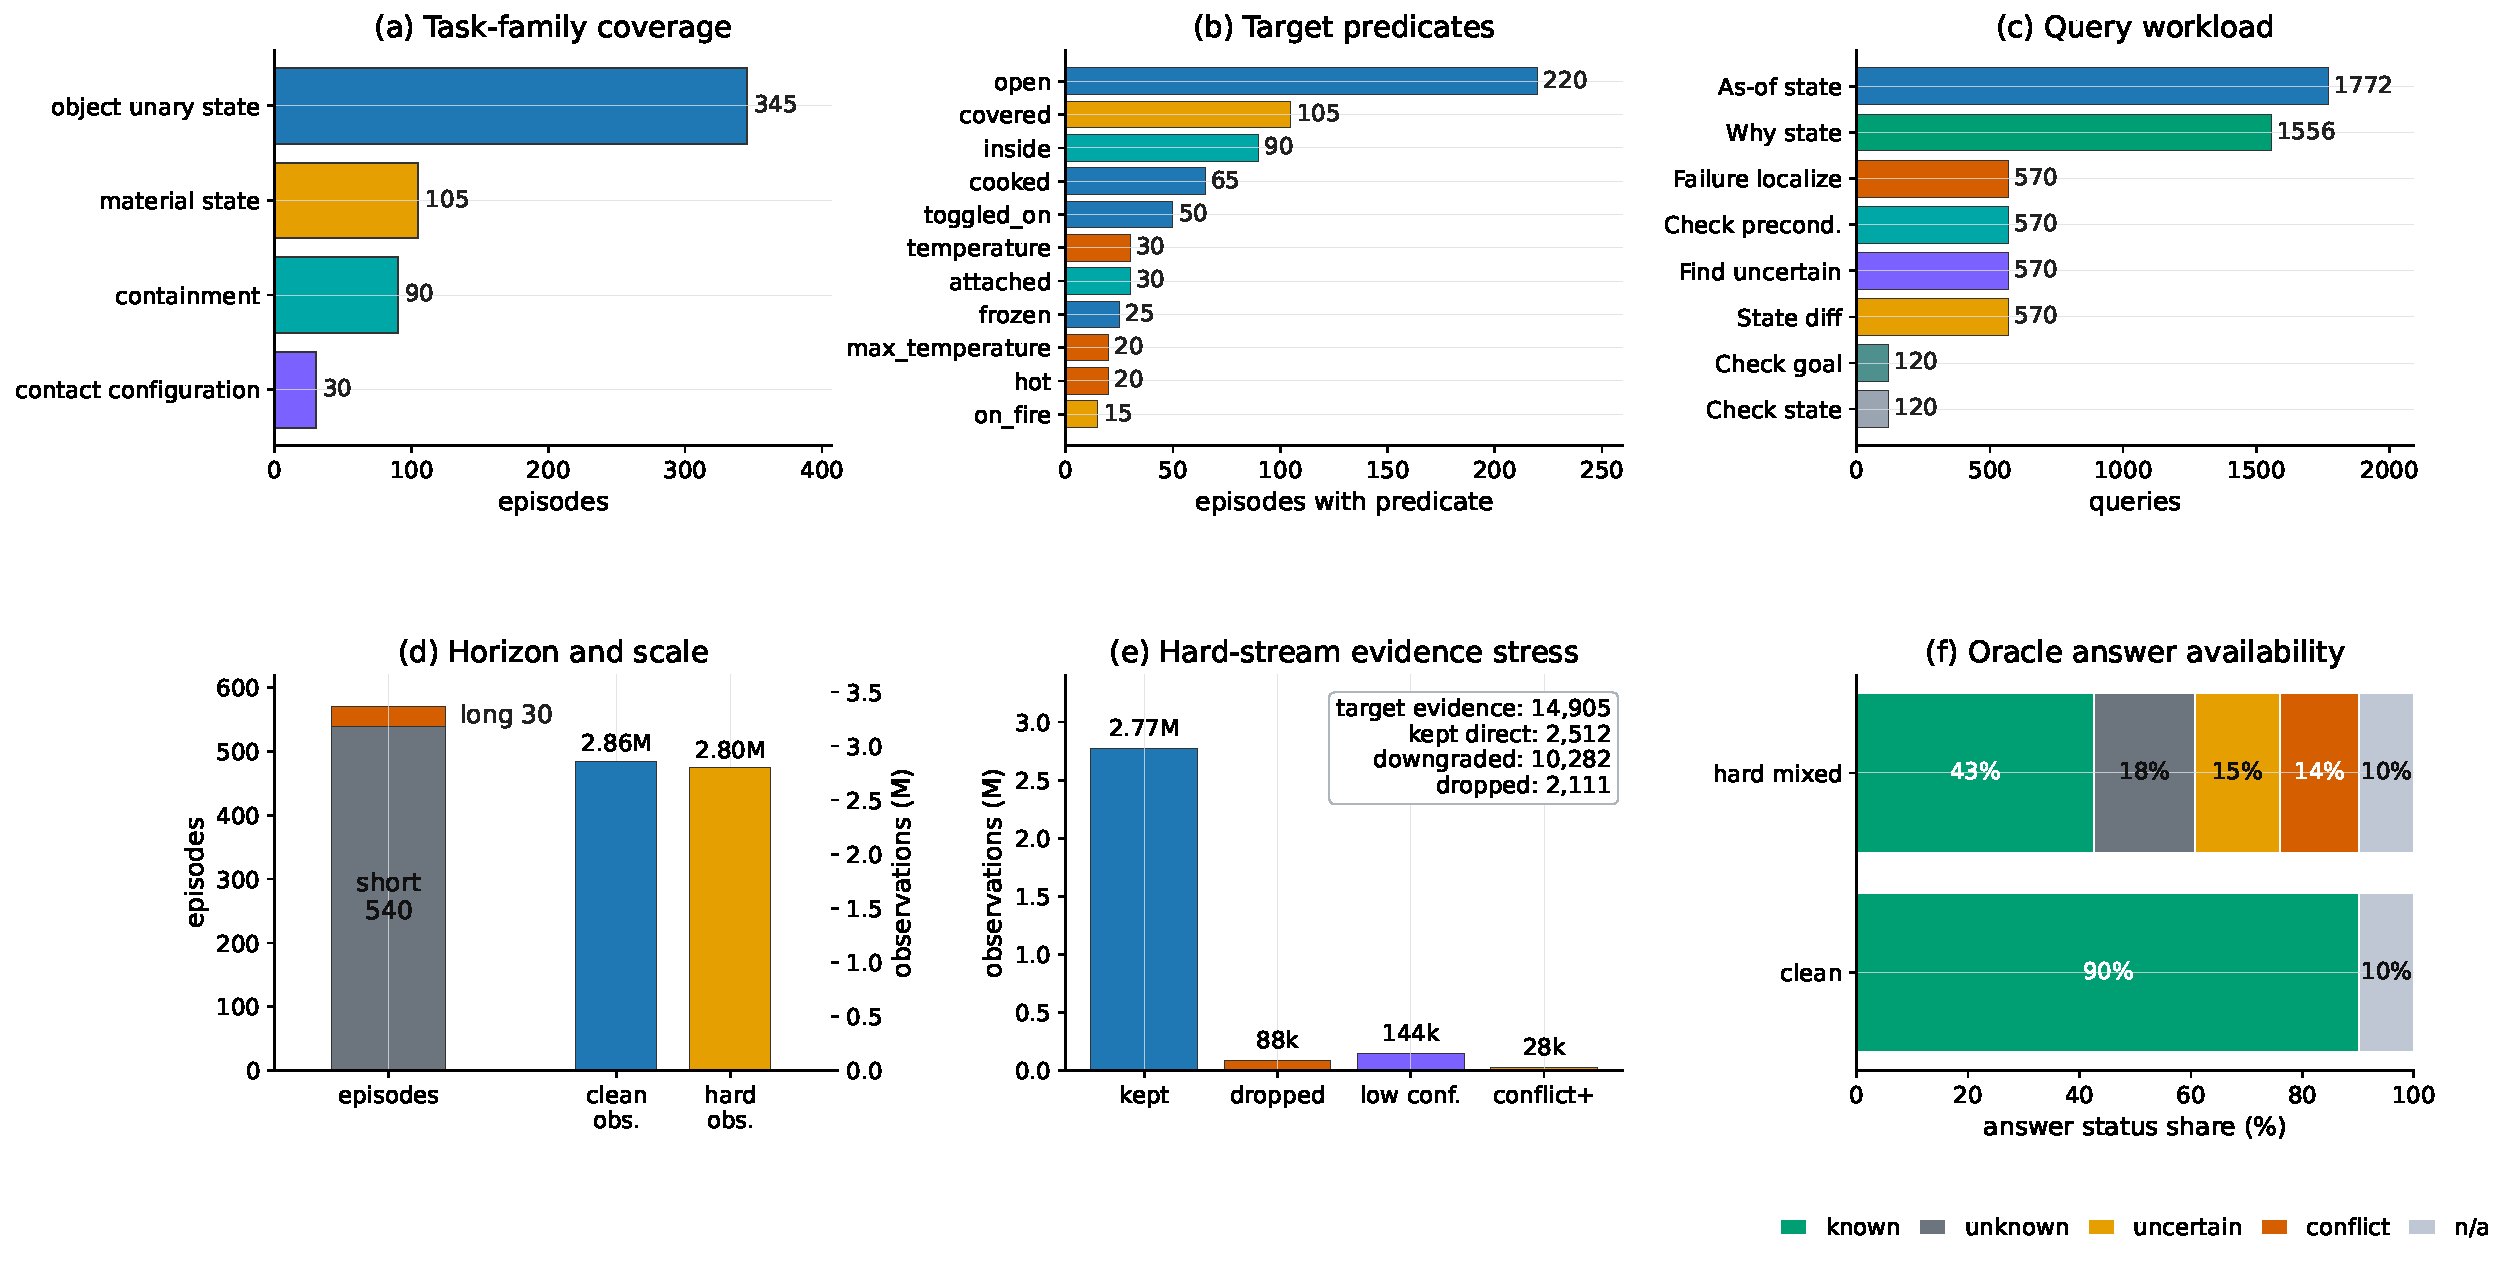
\includegraphics[width=\textwidth]{figures/figA_benchmark_profile.pdf}
\caption{Benchmark artifact profile. \bench\ covers 570 simulator-grounded episodes over 36 activities, four task-state families, and 11 target predicates. The hard mixed stream stresses target evidence and shifts answer availability from mostly known clean answers to a mixture of known, unknown, uncertain, conflicting, and not-applicable answers.}
\label{fig:artifact-profile}
\end{figure*}

\subsection{Artifact Characterization}

The reported artifact supports the first EAB claim: \bench\ is a concrete, validated benchmark package rather than only a proposal. Fig.~\ref{fig:artifact-profile} summarizes the released workload. The artifact contains 570 simulator-grounded episodes, 36 activities, four task-state families, 11 target predicates, 5,848 hard queries, 2.86M clean observations, and 2.80M hard mixed observations. The query set covers point state checks, bitemporal as-of probes, provenance queries, full-episode diffs, uncertainty sets, preconditions, failure localization, and task-goal checks. The target predicates cover object unary state, material state, containment, and contact configuration. This diversity is important because a benchmark limited to one predicate family would be easy to overfit with a specialized rule.

\begin{figure*}[!t]
\centering
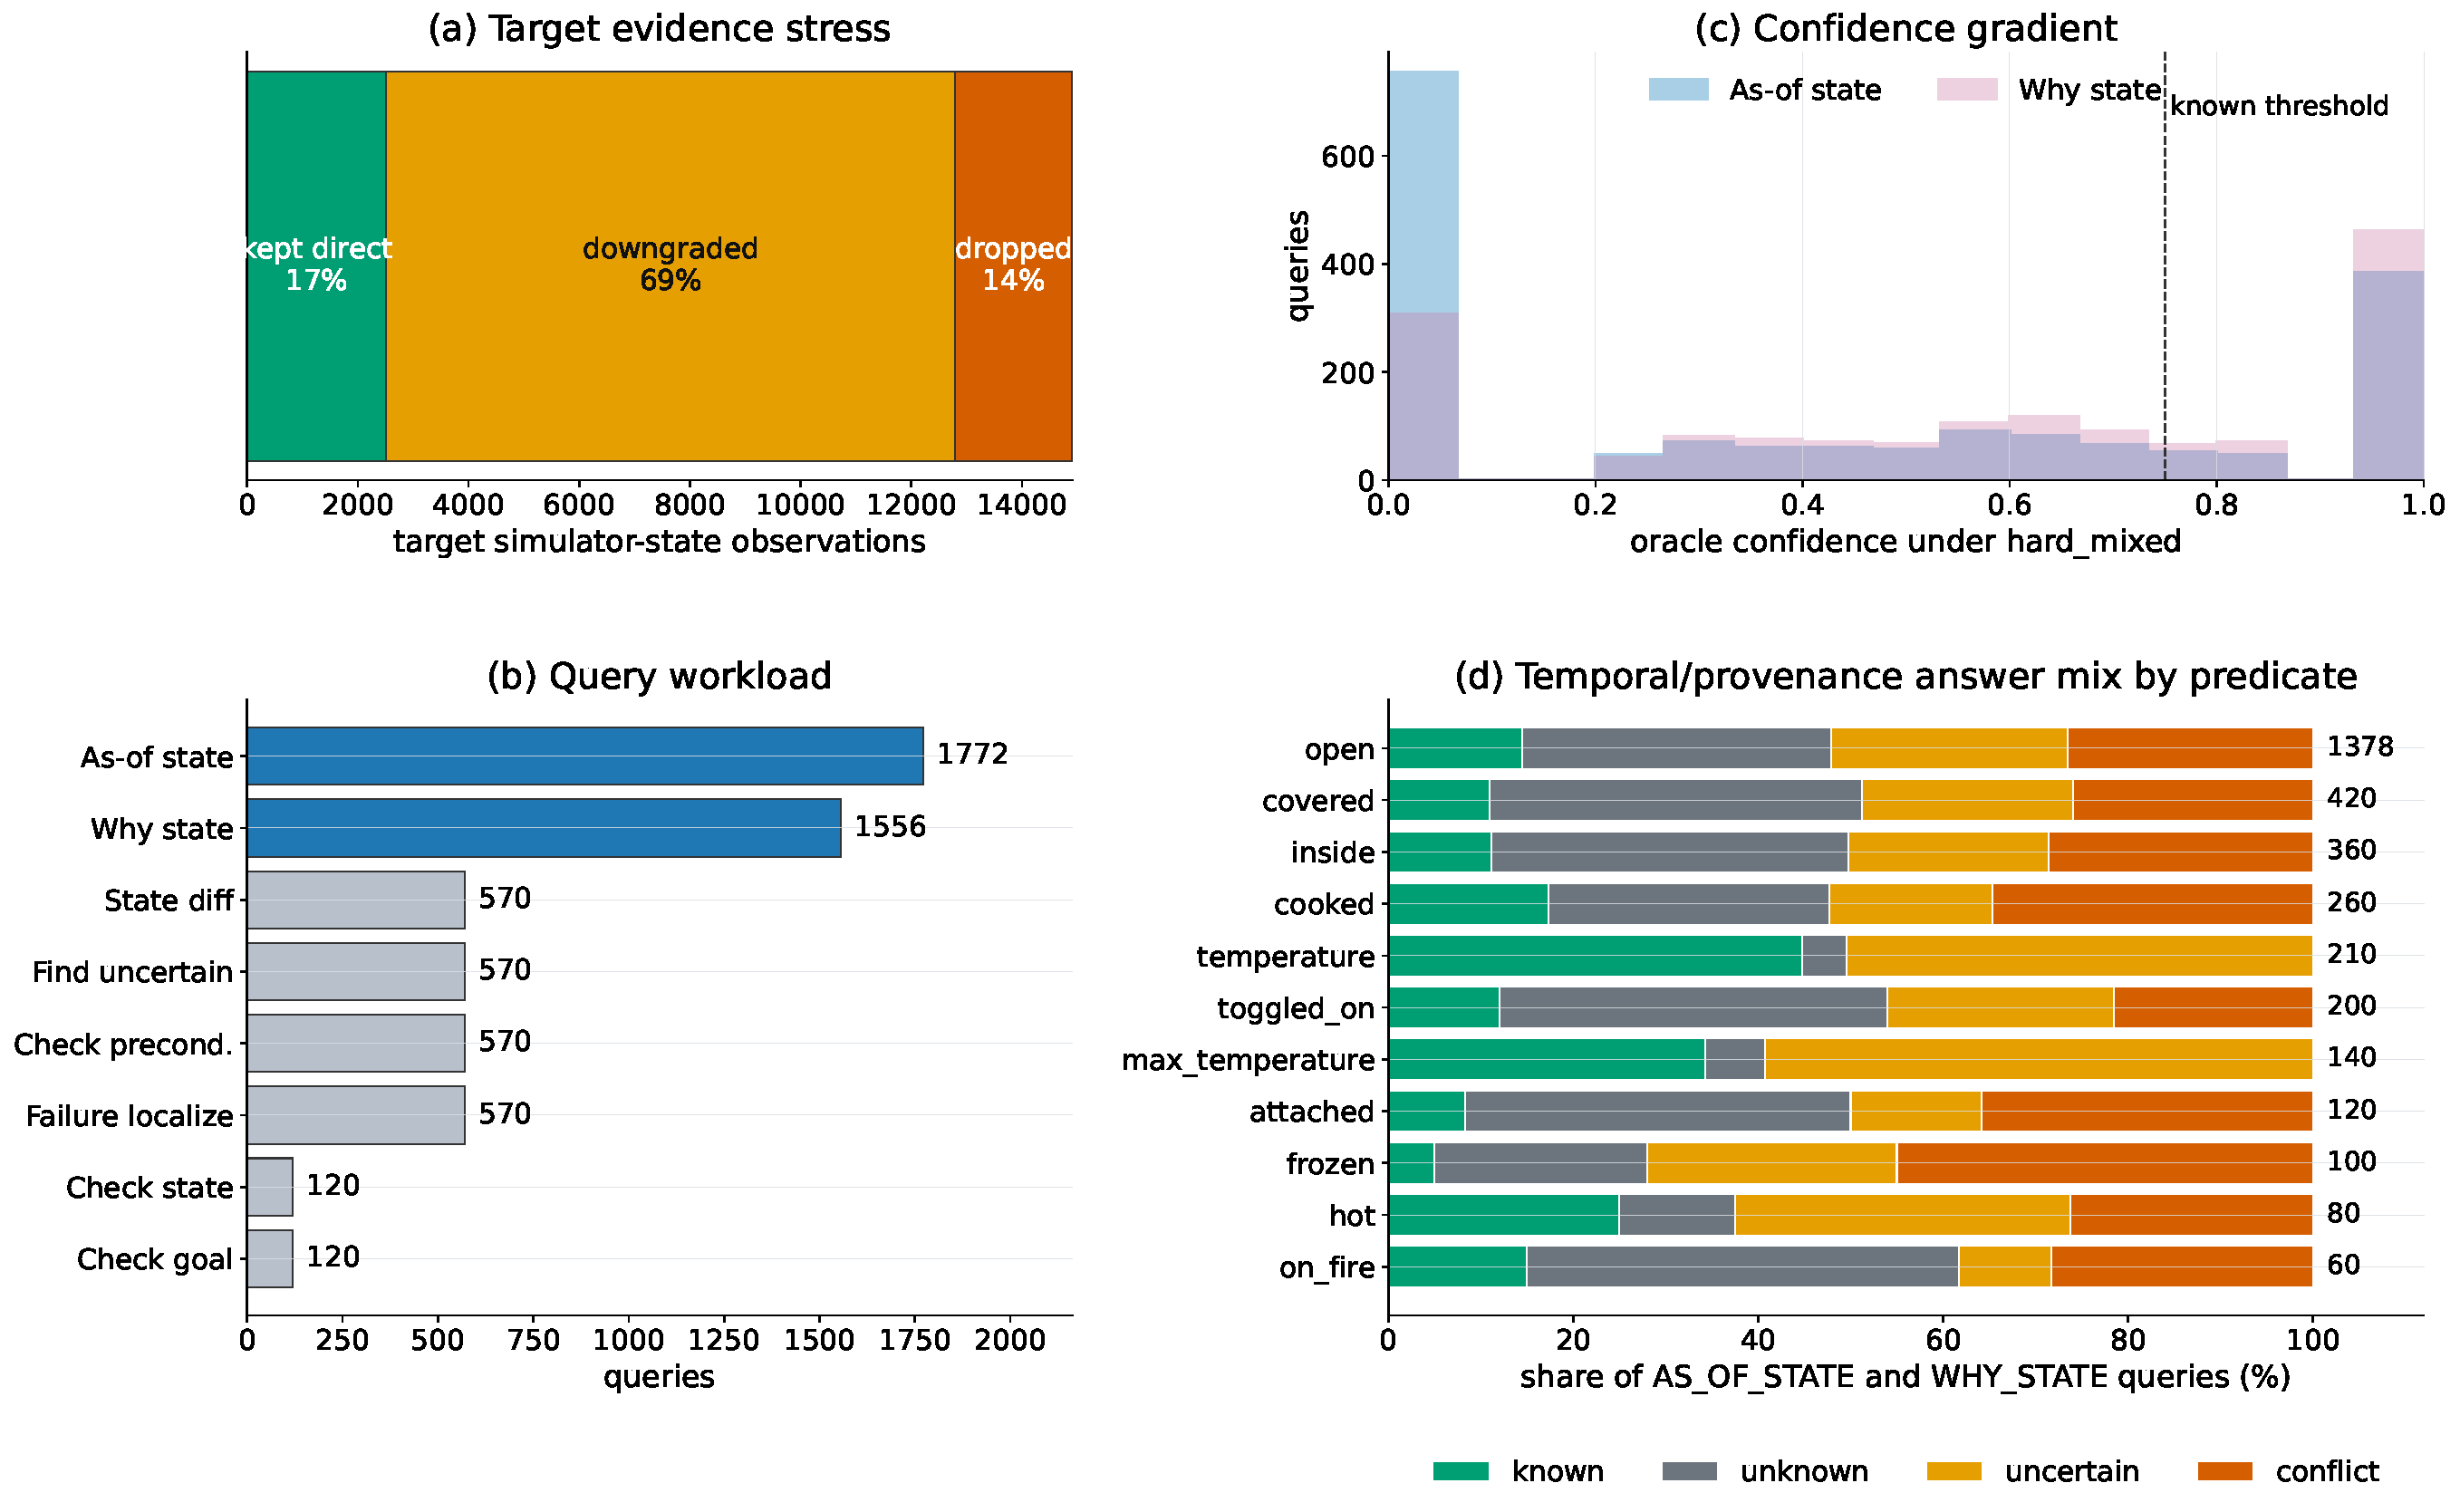
\includegraphics[width=\textwidth]{figures/figB_query_difficulty_matrix.pdf}
\caption{Hard-split mechanism and query difficulty profile. The hard stream keeps only a minority of target simulator-state observations as direct evidence, while downgrading or dropping the rest. The resulting workload emphasizes temporal and provenance queries and produces graded known, unknown, uncertain, and conflicting answer conditions across target predicates.}
\label{fig:hard-profile}
\end{figure*}

\subsection{Hard-Split Difficulty}

Fig.~\ref{fig:hard-profile} explains why the hard split is more than a larger file. Among 14,905 target simulator-state observations, only 2,512 remain as direct target evidence, 10,282 are downgraded to lower-confidence evidence, and 2,111 are dropped. The overall stream also contains 87,571 dropped observations, 144,011 low-confidence observations, and 27,883 injected conflicts. This perturbation is target-aware: it stresses evidence near the states that queries ask about, while leaving most background observations intact.

The hard split is therefore a controlled stress test for data-management behavior. It is not an empirical model of every real sensor failure. Its purpose is to create missing, low-confidence, delayed, and conflicting evidence regimes in which systems must decide whether a state is known, unknown, uncertain, or conflicting. The confidence and predicate panels in Fig.~\ref{fig:hard-profile} show that the resulting workload is not binary. Different predicates exhibit different answer mixtures, and temporal/provenance queries include high-confidence, low-confidence, missing, and conflicting cases.

\subsection{Long State Chains}

Most episodes in the reported artifact are short controlled transitions, but the release also includes a 30-episode long state-chain subset over cooking and freezing activities. The cooking chains move from an actuator state to temperature and maximum-temperature changes, and then to hot and cooked states. The freezing chain moves from opening the refrigerator to temperature change and then to frozen state. This subset is not large enough to claim broad long-horizon BEHAVIOR coverage, but it demonstrates that the benchmark can express multi-stage temporal state maintenance beyond a single target flip.

\begin{figure*}[!t]
\centering
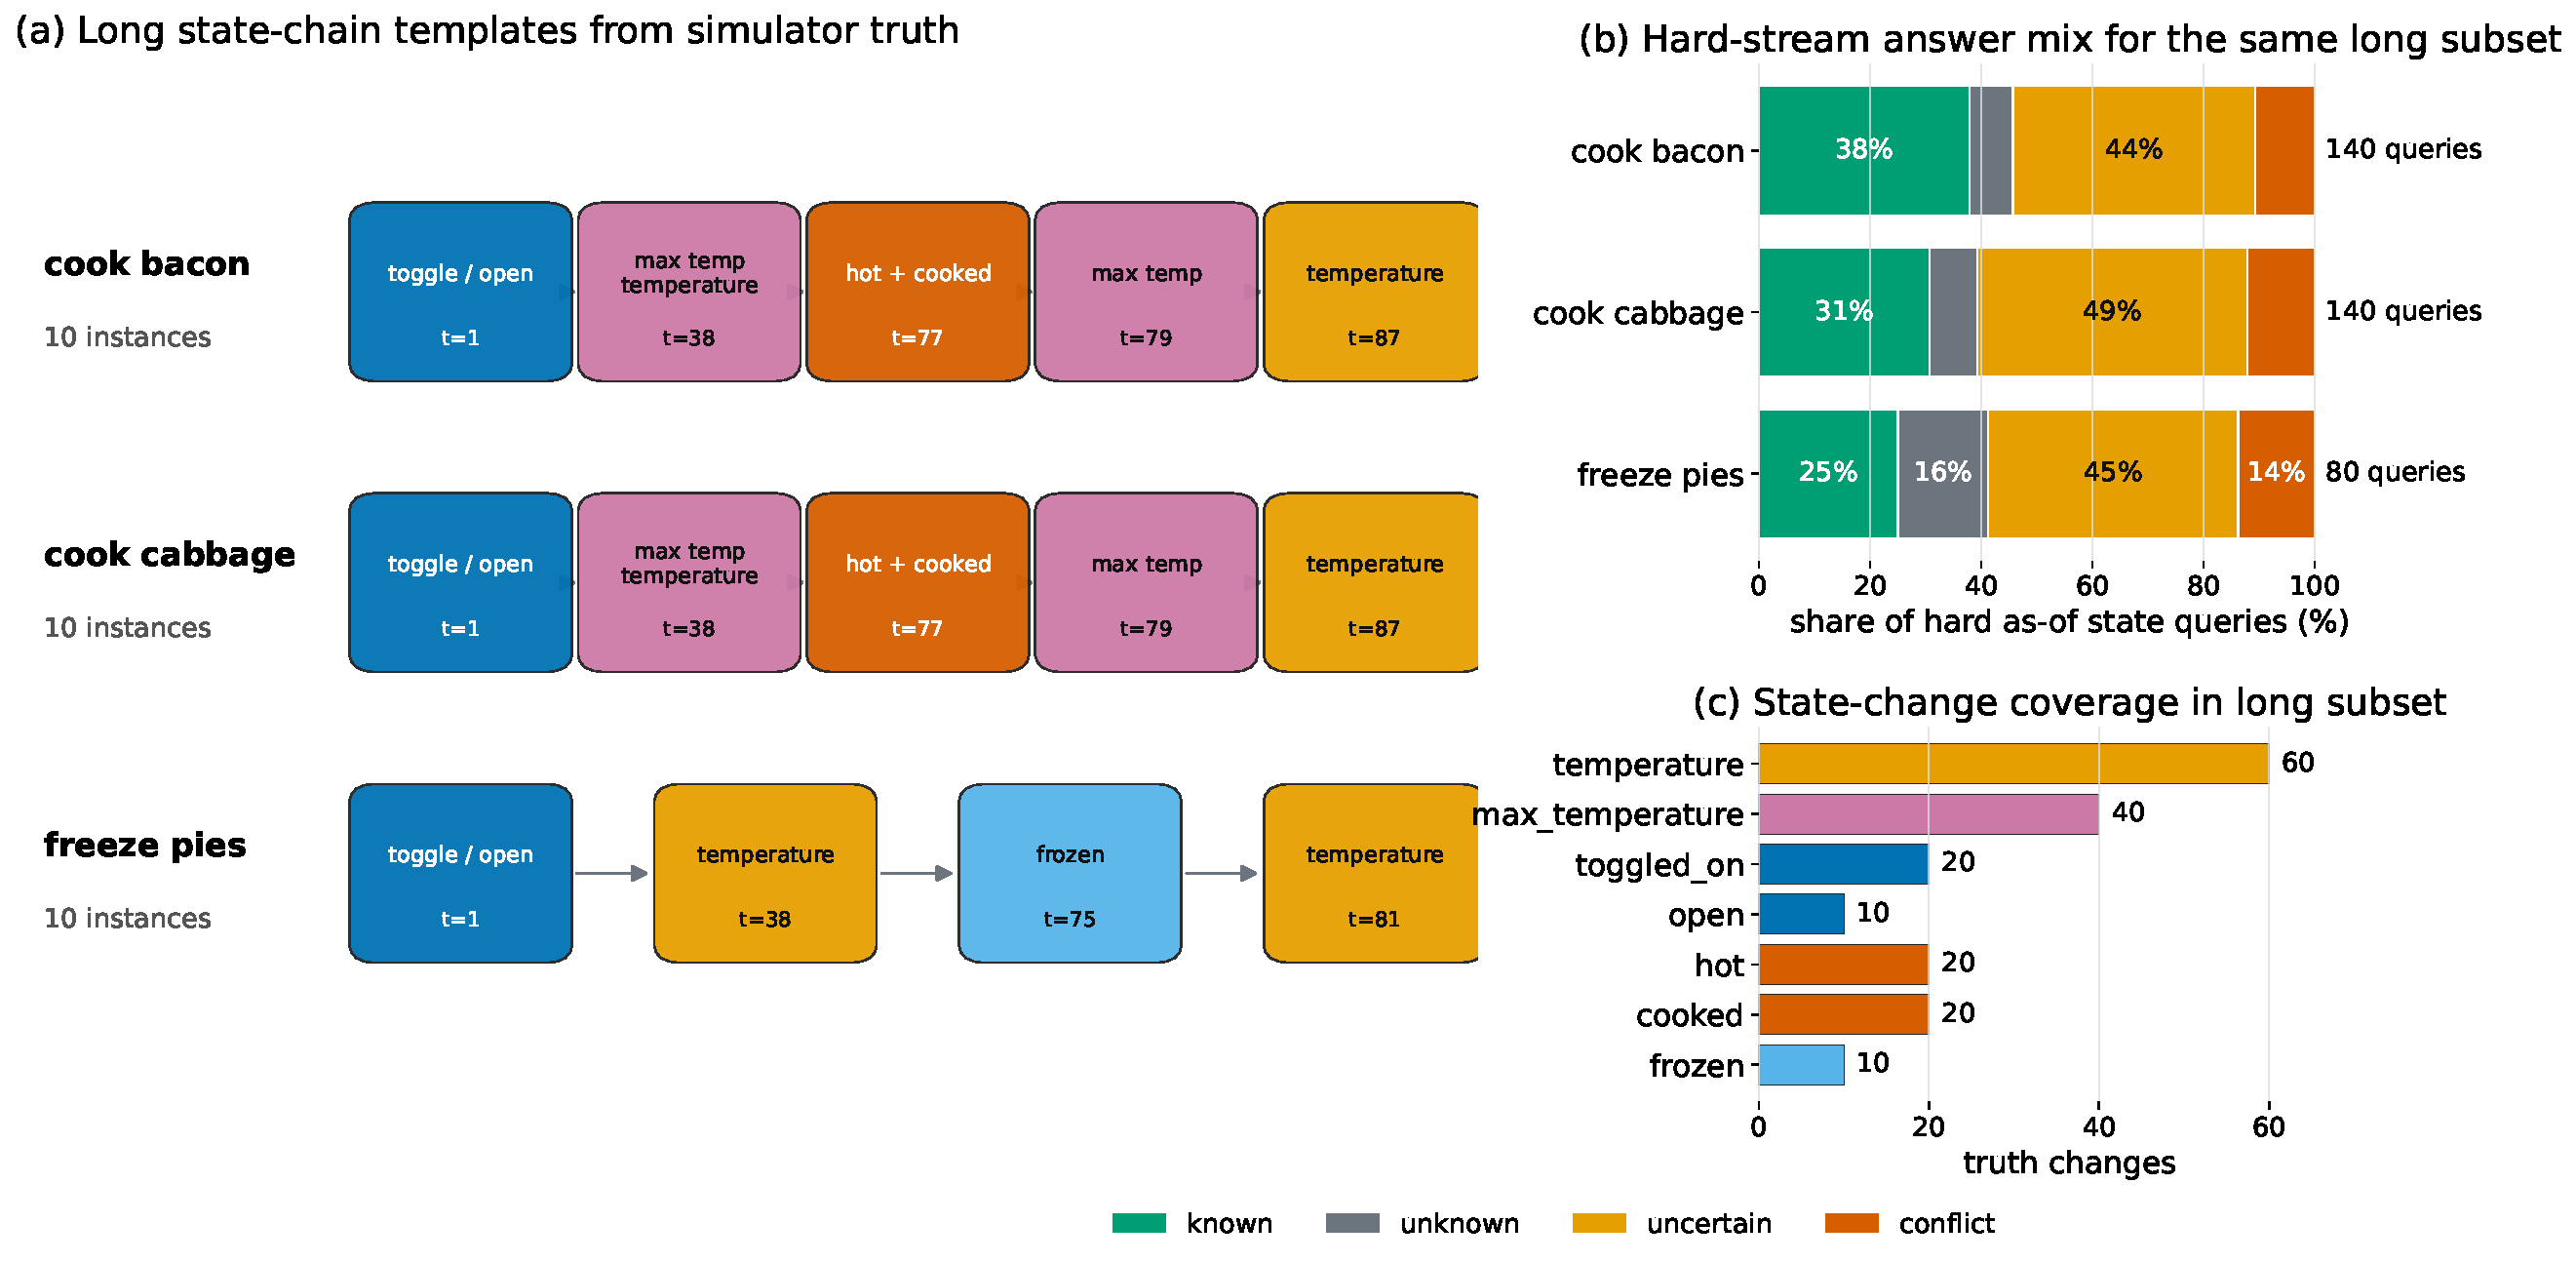
\includegraphics[width=0.84\textwidth]{figures/figC_long_state_chain_timeline.pdf}
\caption{Aggregated long state-chain templates. The 30-episode long subset adds multi-stage temporal maintenance cases, such as actuator, temperature, hot, cooked, and frozen state chains, to the larger short-transition benchmark.}
\label{fig:long-chain}
\end{figure*}

Fig.~\ref{fig:long-chain} makes this diagnostic role explicit. The long subset is small and is not a separate robotics claim; it shows that the artifact can express chained state consequences and convert them into temporal availability cases under hard mixed evidence.

\begin{figure*}[!t]
\centering
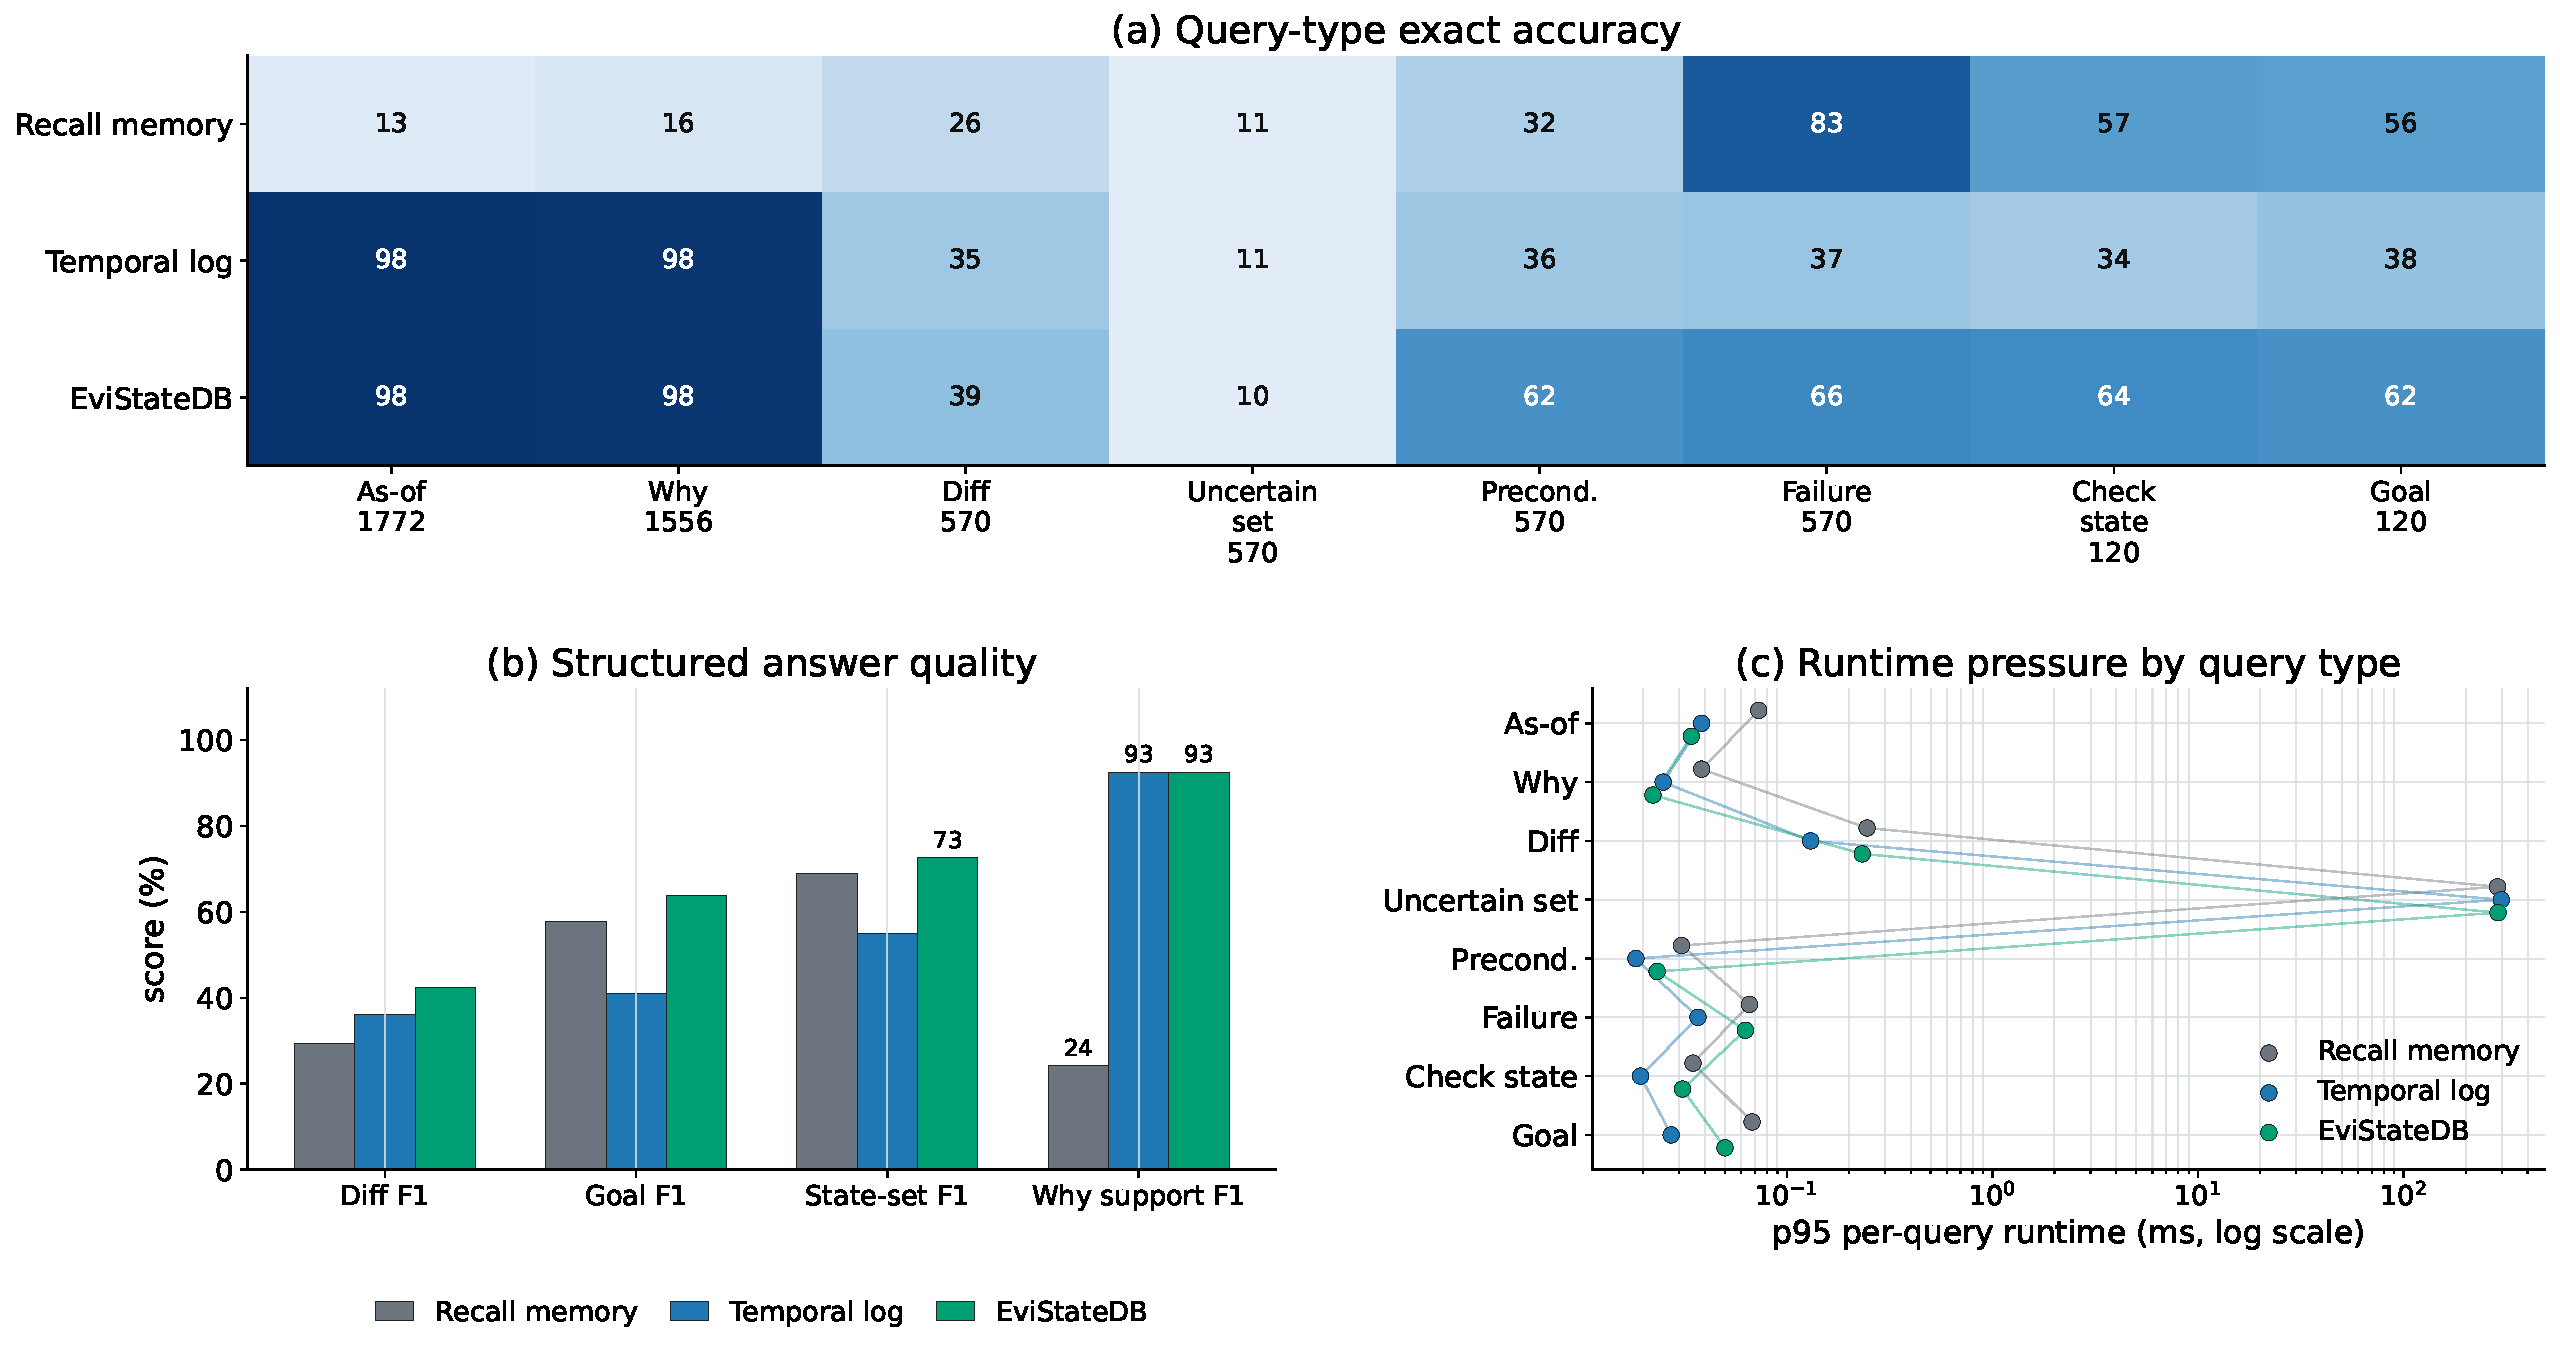
\includegraphics[width=\textwidth]{figures/figD_baseline_main_results.pdf}
\caption{Baseline results on the final hard split. The upper heatmap reports query-type exact accuracy, the lower-left panel reports structured answer metrics, and the lower-right panel reports p95 per-query runtime from prediction outputs. All methods cover the full 5,848-query workload.}
\label{fig:baseline-results}
\end{figure*}

\subsection{Baseline Results}

Fig.~\ref{fig:baseline-results} compares three reference baselines on the final hard split. Recall memory answers from retrieved or recent evidence without maintaining a temporal state view. Temporal log keeps an explicit event log and evaluates temporal queries over it. \engine\ maintains a bitemporal task-state view with support and contradict evidence.

The overall exact accuracies are 25.2\% for Recall memory, 69.0\% for Temporal log, and 75.6\% for \engine. These results support the benchmark's diagnostic goal: the workload separates retrieval-style memory, append-only temporal lookup, and materialized temporal-state views. The largest gap is between retrieval-style memory and the two temporal baselines; the additional gain from Temporal log to \engine\ is smaller and concentrates in structured and task-derived workloads. Temporal log and \engine\ reach 98\% exact accuracy on \texttt{AS\_OF\_STATE} and \texttt{WHY\_STATE}, but they still struggle on structured workloads. \engine\ reaches only 39\% exact accuracy on \texttt{STATE\_DIFF} and 10\% on \texttt{FIND\_UNCERTAIN\_STATES}, although its partial structured metrics are higher: 42.4\% Diff F1, 63.8\% Goal F1, 72.6\% State-set F1, and 92.5\% Why-support F1.

The runtime panel reports per-query prediction time, not full end-to-end indexing or stream-loading time. It shows a different stress point: most point-state queries are inexpensive after indexing, while \texttt{FIND\_UNCERTAIN\_STATES} dominates p95 query time for all methods. This is useful benchmark information because it separates semantic difficulty from query-time pressure.

\subsection{Failure and Difficulty Diagnostics}

The baseline diagnostics separate two different messages. First, answer status matters. Recall memory fails especially on unknown, uncertain, and conflict answers, while Temporal log and \engine\ recover most unknown and uncertain statuses. Second, the high predicate-level accuracy for Temporal log and \engine\ on \texttt{AS\_OF\_STATE} and \texttt{WHY\_STATE} should not be overstated. It means that explicit event-time and transaction-time maintenance is effective for these two query families. It does not mean that all of \bench\ is easy, because the residual errors in Fig.~\ref{fig:baseline-results} concentrate in set-valued uncertainty, state diffs, preconditions, failure localization, and goal views.

\begin{figure*}[!t]
\centering
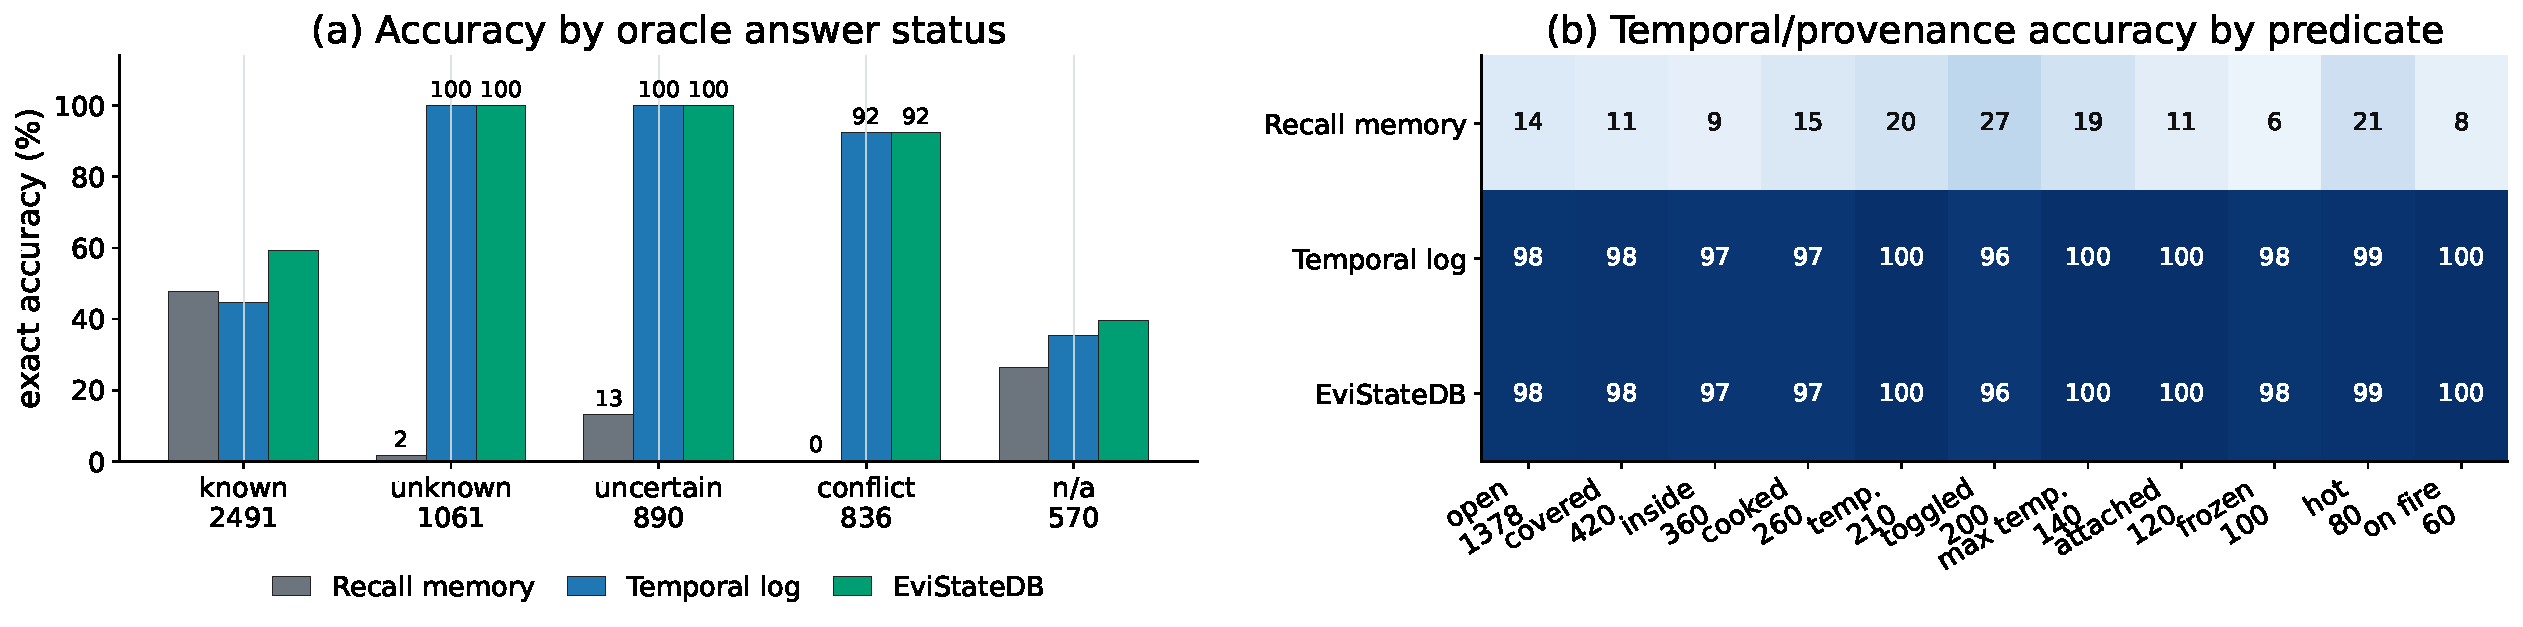
\includegraphics[width=0.84\textwidth]{figures/figE_failure_difficulty_analysis.pdf}
\caption{Difficulty analysis by answer status and predicate. Recall memory degrades across answer statuses and target predicates, while explicit temporal-state baselines largely solve \texttt{AS\_OF\_STATE} and \texttt{WHY\_STATE}.}
\label{fig:failure-diagnostics}
\end{figure*}

Fig.~\ref{fig:failure-diagnostics} explains where residual difficulty comes from. Retrieval fails broadly, while Temporal log and \engine\ largely recover temporal and provenance answers. The remaining difficulty is therefore concentrated in answer shapes that require sets, diffs, preconditions, failure localization, and goal aggregation.

The interpretation should avoid two common mistakes. It should not treat \engine\ as the oracle merely because it is the reference engine. It should also not claim that a lower score means a method is bad for all embodied AI tasks. A retrieval memory that performs poorly on state diffs may still be useful for open-ended question answering. The EAB claim is narrower and more useful: \bench\ identifies which systems are good at temporal task-state view maintenance under a shared, reproducible workload.

\section{Lessons, Limitations, and Artifact Availability}
\label{sec:discussion}

\subsection{Lessons from the Benchmark Design}

\bench\ exposes five practical lessons. First, latest-state memory is not a sufficient abstraction because late evidence can revise as-of answers and contradict evidence can make a state uncertain or conflicting. Second, retrieval and view maintenance answer different questions: retrieval can surface evidence, but task execution often needs a maintained predicate value, change set, or goal view. Third, provenance should be first-class because support and contradict evidence are needed for why queries, failure localization, and trust calibration. Fourth, goal views are not just convenience layers; they can fail even when individual predicates are partly correct. Fifth, validation reports are benchmark artifacts, since malformed query metadata or leaked answer fields can invalidate comparisons as much as model errors.

\subsection{Limitations}

\bench\ makes a controlled isolation choice. The main artifact is simulator-grounded and structured; it does not claim to solve raw perception or low-level robot control. This is a limitation, but also a design requirement for a reproducible data-management benchmark, because folding perception and control into the main score too early would make failures hard to attribute. The reported baseline set is also intentionally conservative: neural memory, LLM-based agents, and full embodied pipelines fit the benchmark only when their public inputs, inference budgets, and output schemas can be made comparable.

\subsection{Artifact Availability}

The benchmark release provides public task specifications, observation streams, query sets, manifests, validation reports, build commands, baseline implementations, prediction schemas, and evaluator scripts. Hidden timelines and answer sets are used for evaluation. The minimal reproduction path builds or validates public artifacts, runs each baseline on the hard mixed stream, validates prediction schema, evaluates predictions, and regenerates the reported tables and figures.

\section{Related Work}
\label{sec:related}

\subsection{Embodied Task and Simulation Benchmarks}

BEHAVIOR introduced a benchmark of everyday household activities with predicate-logic activity specifications and simulation-based evaluation~\cite{srivastava2022behavior}. BEHAVIOR-1K scales this line of work to 1,000 activities and introduces OmniGibson as a simulation environment for realistic physics and rendering~\cite{li2024behavior1k}. Habitat and Habitat 2.0 support embodied navigation and rearrangement evaluation~\cite{savva2019habitat,szot2021habitat}; AI2-THOR provides an interactive 3D environment for visual AI~\cite{kolve2017ai2thor}; VirtualHome represents household activities as executable programs~\cite{puig2018virtualhome}; and TEACh studies embodied agents that interact through dialogue~\cite{padmakumar2022teach}. \bench\ uses the same general idea that task specifications and simulator truth can ground evaluation, but it changes the target from embodied task success to temporal task-state view maintenance.

ALFRED evaluates instruction following~\cite{shridhar2020alfred}, and OpenEQA evaluates embodied question answering over episodic memory and active exploration~\cite{majumdar2024openeqa}. These benchmarks ask whether an agent can act or answer language questions. \bench\ asks whether a system can maintain and query a temporal state view from imperfect evidence, without prescribing the system's internal memory architecture.

\subsection{Temporal, Stream, and Provenance Data Management}

Temporal databases separate the time when a fact is valid in the modeled world from the time when a database records or knows the fact~\cite{snodgrass1999developing,jensen1999temporal}. Stream systems study continuous processing over arriving data~\cite{babcock2002models,garofalakis2016data}. Incremental view maintenance studies how derived database state can be updated after base changes~\cite{gupta1995maintenance,zhuge1995view}. Provenance and uncertain-data systems address evidence and noisy facts~\cite{green2007provenance,cheney2009provenance,aggarwal2009uncertain,dalvi2007efficient}. \bench\ brings these ideas into embodied task-state maintenance, where event-time and arrival-time mismatch, missing observations, conflicting evidence, and task-derived goal views appear together.

\subsection{Experiment, Analysis, and Benchmark Papers}

Database benchmark and EAB papers often contribute workload models, artifact rules, and diagnostic analyses rather than only a new algorithm. LDBC standardizes graph workloads~\cite{erling2015ldbc,iosup2016ldbc}; TSM-Bench benchmarks time-series systems~\cite{khelifati2023tsmbench}; and FinBench defines a financial graph transaction workload~\cite{qi2025finbench}. Recent EAB papers similarly contribute evaluation frameworks and fine-grained diagnostics, including SQLMorph~\cite{malekpour2026sqlmorph}, BEACON~\cite{najafi2025beacon}, and plan-based AQP analysis~\cite{mu2025aqp}. \bench\ follows this pattern: the contribution is the benchmark artifact, workload, evaluator, and analysis of where baseline strategies succeed or fail.

\section{Conclusion}

\bench\ is a data-management benchmark for temporal task-state view maintenance over embodied observation streams. It separates public observation streams and queries from hidden timelines and answers, evaluates systems through standardized QueryAnswers, and makes event time, arrival time, evidence, perturbations, and task-derived state views first-class benchmark concerns. \engine\ provides a reference baseline engine, but the benchmark oracle comes from simulator truth and task specifications. The reported artifact and experiments show that temporal maintenance strategies outperform retrieval-style memory on this workload, while structured, set-valued, and task-derived queries remain open stress points for submitted systems.

\section*{AI-Generated Content Acknowledgement}

The authors used AI-assisted tools during manuscript drafting, code editing, experiment-log summarization, and figure-preparation support. The authors reviewed, edited, and verified the submitted content and remain responsible for the correctness, originality, and integrity of the paper.

\bibliographystyle{IEEEtran}
\bibliography{refs}

\end{document}
